\documentclass{ximera}

\newcommand{\RR}{\mathbb R}
\renewcommand{\d}{\,d}
\newcommand{\dd}[2][]{\frac{d #1}{d #2}}
\renewcommand{\l}{\ell}
\newcommand{\ddx}{\frac{d}{dx}}
\newcommand{\dfn}{\textbf}
\newcommand{\eval}[1]{\bigg[ #1 \bigg]}


\author{Bart Snapp}


\outcome{State the definition of a vector.}
\outcome{Work with vectors in two or three dimensions. }
\outcome{Multiply vectors by scalars.}
\outcome{Add and subtract vectors.}
\outcome{Calculate the magnitude of a vector.}
\outcome{Find unit vectors.}
\outcome{Use vectors in applied settings.}


\title[Dig-In:]{Vectors}

\begin{document}
\begin{abstract}
  Vectors are lists of numbers that denote direction and magnitude.
\end{abstract}
\maketitle


\section{The idea of vectors}

The most successful textbook that was ever written was
\link[\textit{Euclid's
    Elements}]{https://mathcs.clarku.edu/~djoyce/java/elements/elements.html}. While
you are surely skeptical of this claim, and it is \textit{good} to be
skeptical, consider this: \textit{Euclid's Elements} was used (in
various editions) as a primary mathematics textbook for nearly 2000
years. There are few textbooks (if any) that can share this
claim. However, \textit{Euclid's Elements} does have its short
comings. Euclid defines a point as ``that which has no part.'' That is
a pretty confusing definition. It is not really clear to this author
what Euclid means. However, from our modern viewpoint, a point is an
ordered list of numbers, like:
\[
(1,1)\quad\text{or}\quad(4,2)
\]
We have grown to see that a point should be thought of as
\textit{location}, and nothing but location. With this in mind, it
doesn't really make sense to have operations between points like
adding or subtraction.

When trying to understand the world around us, we are often concerned
with quantities that denote both \textit{direction} and
\textit{magnitude}. We can do this by starting with two points:
\begin{image}
  \begin{tikzpicture}
	\begin{axis}[
            xmin=-1,xmax=5,ymin=-1,ymax=3,
            clip=false,
            axis lines=center,
            ticks=none,
            unit vector ratio*=1 1 1,
            xlabel=$x$, ylabel=$y$,
            %ytick={-2,-1,...,7},
	    %xtick={-2,-1,...,10},
	    %grid = major,
            every axis y label/.style={at=(current axis.above origin),anchor=south},
            every axis x label/.style={at=(current axis.right of origin),anchor=west},
          ]
          \addplot[mark=*,penColor2] coordinates {(1,1)};
          \addplot[mark=*,penColor2] coordinates {(4,2)};
          \node[above] at (axis cs:4, 2) [penColor2] {$(a,b)$};
          \node[below] at (axis cs:1, 1) [penColor2] {$(c,d)$};
        \end{axis}
\end{tikzpicture}
\end{image}
and thinking of the difference of their coordinates:
\begin{image}
  \begin{tikzpicture}
	\begin{axis}[
            xmin=-1,xmax=5,ymin=-1,ymax=3,
            clip=false,
            axis lines=center,
            ticks=none,
            unit vector ratio*=1 1 1,
            xlabel=$x$, ylabel=$y$,
            %ytick={-2,-1,...,7},
	    %xtick={-2,-1,...,10},
	    %grid = major,
            every axis y label/.style={at=(current axis.above origin),anchor=south},
            every axis x label/.style={at=(current axis.right of origin),anchor=west},
          ]
          \addplot[mark=*,penColor2] coordinates {(1,1)};
          \addplot[mark=*,penColor2] coordinates {(4,2)};
          
          \addplot[very thick,penColor,->] plot coordinates {(1,1) (4,2)};
          \node[above] at (axis cs:4, 2) [penColor2] {$\mathrm{tip}=(a,b)$};
          \node[below] at (axis cs:1, 1) [penColor2] {$\mathrm{tail}=(c,d)$};
          \node[below right] at (axis cs:2.5, 1.5) [penColor] {$\vec{v}=\vector{a-c,b-d}$};
        \end{axis}
\end{tikzpicture}
\end{image}
This difference in the values of the coordinates of the points is a
called a \textit{vector}. In the graph above, the vector is
$\vec{v}=\vector{a-c,b-d}$. We write vectors typographically in
boldfaced decorated with a harpoon (like $\vec{v}$ or
$\vec{w}$). Other authors may simply used a boldface (like
$\mathbf{v}$ or $\mathbf{w}$) or just a harpoon (like $\arrowvec{v}$
or $\arrowvec{w}$). We often visualize a vector (at least in two and
three dimensions) as an arrow to explicitly show its direction and
magnitude. This leads us to our definition of a vector:

\begin{definition}
  A \dfn{vector} is something that can be ascribed the qualities of
  direction and magnitude. 
\end{definition}

\begin{question}
  What vector has its tip at $(1,2)$ and its tail at $(4,3)$?
  \begin{prompt}
    \[
    \vec{v} = \vector{\answer{-3},\answer{-1}}
    \]
  \end{prompt}
  
  \begin{feedback}[correct]
    Note, since we are denoting the vector by a single pair of
    numbers, this pair of numbers represents the tip of the vector,
    and we assume that the tail of the vector is at the origin:
     \begin{image}
       \begin{tikzpicture}
	 \begin{axis}[
            xmin=-4,xmax=5,ymin=-2,ymax=4,
            clip=false,
            axis lines=center,
            %ticks=none,
            unit vector ratio*=1 1 1,
            xlabel=$x$, ylabel=$y$,
            ytick={-2,-1,...,4},
	    xtick={-4,-3,...,5},
	    grid = major,
            every axis y label/.style={at=(current axis.above origin),anchor=south},
            every axis x label/.style={at=(current axis.right of origin),anchor=west},
          ]
          \addplot[very thick,penColor,->] plot coordinates {(4,3) (1,2)};
          \addplot[very thick,penColor2,->] plot coordinates {(0,0) (-3,-1)};
          \node[above] at (axis cs:2.5, 2.5) [penColor] {$\vec{v}$};
          \node[above] at (axis cs:-1.5, -.5) [penColor2] {$\vec{v}$};

         \end{axis}
       \end{tikzpicture}
     \end{image}
  \end{feedback}
\end{question}
Two vectors are equal when they have the same direction and magnitude.
\begin{question}
  True or False: Given vectors $\vec{v}$ and $\vec{w}$ in the diagram
  below
  \begin{image}
  \begin{tikzpicture}
	\begin{axis}[
            xmin=-1,xmax=5,ymin=-1,ymax=4,
            clip=false,
            axis lines=center,
            %ticks=none,
            unit vector ratio*=1 1 1,
            xlabel=$x$, ylabel=$y$,
            %ytick={-2,-1,...,7},
	    %xtick={-2,-1,...,10},
	    grid = major,
            every axis y label/.style={at=(current axis.above origin),anchor=south},
            every axis x label/.style={at=(current axis.right of origin),anchor=west},
          ]
          \addplot[very thick,penColor,->] plot coordinates {(1,2) (4,3)};
          \addplot[very thick,penColor2,->] plot coordinates {(0,0) (3,1)};
          \node[above] at (axis cs:2.5, 2.5) [penColor] {$\vec{v}$};
          \node[above] at (axis cs:1.5, .5) [penColor2] {$\vec{w}$};

        \end{axis}
\end{tikzpicture}
\end{image}
  we have that $\vec{v}=\vec{w}$.
  \begin{prompt}
  \begin{multipleChoice}
    \choice[correct]{true}
    \choice{false}
  \end{multipleChoice}
  \end{prompt}
\end{question}

Vector need not be limited to the $(x,y)$-plane. They can have any \textit{dimension}.

\begin{definition}
The \dfn{dimension} of a vector is the number of entries. Each
individual entry of a vector is called a \dfn{component}.
\end{definition}

In $\R^2$ we usually label the first component the ``$x$-component,''
and the second component the ``$y$-component.'' In $\R^3$ we usually
label the components ``$x$,'' ``$y$,'' and ``$z$.''


\begin{question}
  What is the dimension of the vector 
  \[
  \vector{3,4,1,-4}?
  \]
  \begin{prompt}
  \[
  \text{Dimension} = \answer{4}
  \]
  \end{prompt}
  \begin{question}
    What are the components of the vector $\vector{1,2,3}$?
    \begin{prompt}
      \begin{itemize}
      \item The $x$-component is $\answer{1}$.
      \item The $y$-component is $\answer{2}$.
      \item The $z$-component is $\answer{3}$.
      \end{itemize}
    \end{prompt}
  \end{question}
\end{question}


So far, we have mostly studied functions which take single numbers as
their inputs and output either individual numbers or ordered-pairs (as
in the case of parametric functions).  Now we set the stage for the
study of functions that accept lists of numbers as inputs and lists of
numbers as outputs. When we want to keep track of more than one number
at a time, we often use a vector.



\subsection{Computing the direction and magnitude of vectors}


Since vectors are determined only by their direction and magnitude,
notation such as
\[
\vector{a,b,c}
\]
completely describes a vector, since we assume the tail is at the
origin. We should point out that there is other notation for vectors:
\[
\begin{bmatrix}
  a\\
  b\\
  c
\end{bmatrix}, \quad
\begin{bmatrix}
  a & b & c
\end{bmatrix},
\quad
(a,b,c).
\]
When dealing with a vector in $1$, $2$, or $3$ dimensions, we can
visualize the vector as a directed arrow, where the \textit{magnitude}
is the length of the arrow.

\begin{question}
  What is the magnitude of the vector $\vector{1,1}$?
  \begin{prompt}
    \[
    \text{Magnitude}  = \answer{\sqrt{2}}
    \]
  \end{prompt}
\end{question}

You were able to find the answer to the question above because you are
used to working with $2$ dimensional objects.  We make the following
definition in $n$ dimensions.

\begin{definition}
	Let $\vec{v} = \vector{v_1, v_2, v_3, \dots, v_n}$ in $\R^n$
        be an $n$-dimensional vector.  Then the \dfn{magnitude} of
        $\vec{v}$ is denoted by $|\vec{v}|$ and is defined by:
	\[
	|\vec{v}| = \sqrt{v_1^2+v_2^2+v_3^2+\dots+v_n^2}
	\]
\end{definition}

Note, the magnitude of the vector is just the distance of the point
determined by its components from the origin!

\begin{question}
  What is the magnitude of the vector
  \[
  \vec{v}=\vector{2,-1,4,-2}?
  \]
  \begin{prompt}
    \[
    |\vec{v}|=\answer{5}
    \]
  \end{prompt}
\end{question}




\section{Operations on vectors}


We can add vectors of the same dimension together by component-wise
addition. Here it is useful to write vectors vertically:
\[
\begin{bmatrix}
  a\\
  b\\
  c
\end{bmatrix}
+
\begin{bmatrix}
  d\\
  e\\
  f
\end{bmatrix}
=
\begin{bmatrix}
  a+d\\
  b+e\\
  c+f
\end{bmatrix}.
\]

\begin{question}
  \[
  \vector{1,2,3}+ \vector{-1,2,2} =
  \vector{\answer{0},\answer{4},\answer{5}}
  \]
\end{question}

Now let us investigate the geometry of addition of vectors. Let
$\vec{v} = \vector{1,2}$ and $\vec{w} = \vector{3,1}$.  If we
place the tail of the vector $\vec{w}$ at the tip of the vector
$\vec{v}$, like this:
\begin{image}
  \begin{tikzpicture}
    \begin{axis}[
        xmin=-1,xmax=5,ymin=-1,ymax=4,
            axis lines=center,
            %ticks=none,
            unit vector ratio*=1 1 1,
            xlabel=$x$, ylabel=$y$,
            ytick={-2,-1,...,7},
	    %yticklabels={$0.5$,$1$,$1.5$,$2$},
	    xtick={-2,-1,...,10},
	    %xticklabels={$0.5$,$1$,$1.5$,$2$},
	    grid = major,
            every axis y label/.style={at=(current axis.above origin),anchor=south},
            every axis x label/.style={at=(current axis.right of origin),anchor=west},
          ]
          \addplot[very thick,penColor,->] plot coordinates {(1,2) (4,3)};
          \addplot[very thick,penColor2,->] plot coordinates {(0,0) (1,2)};
          \addplot[ultra thick,penColor3,->] plot coordinates {(0,0) (4,3)};

           \node[left] at (axis cs:.5, 1) [penColor2] {$\vec{v}$};
           \node[above] at (axis cs:2.5, 2.5 ) [penColor] {$\vec{w}$};
           \node[below right] at (axis cs:2, 1.5 ) [penColor3] {$\vec{v}+\vec{w}$};
    \end{axis}
\end{tikzpicture}
\end{image}
Or like this:
\begin{image}
  \begin{tikzpicture}
    \begin{axis}[
        xmin=-1,xmax=5,ymin=-1,ymax=4,
            axis lines=center,
            %ticks=none,
            unit vector ratio*=1 1 1,
            xlabel=$x$, ylabel=$y$,
            ytick={-2,-1,...,7},
	    %yticklabels={$0.5$,$1$,$1.5$,$2$},
	    xtick={-2,-1,...,10},
	    %xticklabels={$0.5$,$1$,$1.5$,$2$},
	    grid = major,
            every axis y label/.style={at=(current axis.above origin),anchor=south},
            every axis x label/.style={at=(current axis.right of origin),anchor=west},
          ]
          \addplot[very thick,penColor2,->] plot coordinates {(3,1) (4,3)};
          \addplot[very thick,penColor3,->] plot coordinates {(0,0) (4,3)};
          \addplot[ultra thick,penColor,->] plot coordinates {(0,0) (3,1)};

           \node[right] at (axis cs:3.5, 2) [penColor2] {$\vec{v}$};
           \node[below] at (axis cs:1.5, .5 ) [penColor] {$\vec{w}$};
           \node[above left] at (axis cs:2, 1.5 ) [penColor3] {$\vec{v}+\vec{w}$};
    \end{axis}
\end{tikzpicture}
\end{image}
then the sum $\vec{v}+\vec{w}$ connects the tail of $\vec{v}$ to the
tip of $\vec{w}$. In fact, you can think of the sum of two vectors as
being the diagonal of the parallelogram formed by the two vectors:
\begin{image}
  \begin{tikzpicture}
    \begin{axis}[
        xmin=-1,xmax=5,ymin=-1,ymax=4,
            axis lines=center,
            %ticks=none,
            unit vector ratio*=1 1 1,
            xlabel=$x$, ylabel=$y$,
            ytick={-2,-1,...,7},
	    %yticklabels={$0.5$,$1$,$1.5$,$2$},
	    xtick={-2,-1,...,10},
	    %xticklabels={$0.5$,$1$,$1.5$,$2$},
	    grid = major,
            every axis y label/.style={at=(current axis.above origin),anchor=south},
            every axis x label/.style={at=(current axis.right of origin),anchor=west},
          ]
          \addplot[very thick,penColor,->] plot coordinates {(1,2) (4,3)};
          \addplot[very thick,penColor2,->] plot coordinates {(0,0) (1,2)};
          \addplot[ultra thick,penColor3,->] plot coordinates {(0,0) (4,3)};

          \node[left] at (axis cs:.5, 1) [penColor2] {$\vec{v}$};
          \node[above] at (axis cs:2.5, 2.5 ) [penColor] {$\vec{w}$};
          \node[below right] at (axis cs:1.9, 1.6 ) [penColor3] {$\vec{v}+\vec{w}$};
          
          \addplot[very thick,penColor2,->] plot coordinates {(3,1) (4,3)};
          \addplot[very thick,penColor3,->] plot coordinates {(0,0) (4,3)};
          \addplot[ultra thick,penColor,->] plot coordinates {(0,0) (3,1)};
          
          \node[right] at (axis cs:3.5, 2) [penColor2] {$\vec{v}$};
          \node[below] at (axis cs:1.5, .5 ) [penColor] {$\vec{w}$};
          %\node[above left] at (axis cs:2, 1.5 ) [penColor3] {$\vec{v}+\vec{w}$};
    \end{axis}
\end{tikzpicture}
\end{image}



Hence
\[
\vec{v}+\vec{w} = \vector{4 , 3}.
\]
\begin{question}
  Consider the following diagram:
  \begin{image}
  \begin{tikzpicture}
    \begin{axis}[
        xmin=0,xmax=5,ymin=-1,ymax=4,
        axis lines=center,
            %ticks=none,
            unit vector ratio*=1 1 1,
            xlabel=$x$, ylabel=$y$,
            ytick={-2,-1,...,7},
	    %yticklabels={$0.5$,$1$,$1.5$,$2$},
	    xtick={-2,-1,...,10},
	    %xticklabels={$0.5$,$1$,$1.5$,$2$},
	    grid = major,
            every axis y label/.style={at=(current axis.above origin),anchor=south},
            every axis x label/.style={at=(current axis.right of origin),anchor=west},
          ]
          \addplot[very thick,penColor,->] plot coordinates {(2,3) (1,0)};
          \addplot[very thick,penColor2,->] plot coordinates {(4,1) (1,0)};
          \addplot[very thick,penColor3,->] plot coordinates {(4,1) (2,3)};
          
          \node[left] at (axis cs:1.5, 1.5 ) [penColor] {$\vec{a}$};
          \node[below] at (axis cs:2.5, .5) [penColor2] {$\vec{b}$};
          \node[above right] at (axis cs:3, 2 ) [penColor3] {$\vec{c}$};
    \end{axis}
  \end{tikzpicture}
  \end{image}
  Which equation is represented by the diagram above?
  \begin{multipleChoice}
    \choice{$\vec{a} + \vec{b} = \vec{c}$}
    \choice[correct]{$\vec{a} + \vec{c} = \vec{b}$}
    \choice{$\vec{b} + \vec{c} = \vec{a}$}
  \end{multipleChoice}
  \begin{feedback}[correct]
    We also could have drawn the diagram above like this:
      \begin{image}
        \begin{tikzpicture}
          \begin{axis}[
              xmin=0,xmax=5,ymin=-1,ymax=4,
              axis lines=center,
              %ticks=none,
              unit vector ratio*=1 1 1,
              xlabel=$x$, ylabel=$y$,
              ytick={-2,-1,...,7},
	      %yticklabels={$0.5$,$1$,$1.5$,$2$},
	      xtick={-2,-1,...,10},
	      %xticklabels={$0.5$,$1$,$1.5$,$2$},
	      grid = major,
              every axis y label/.style={at=(current axis.above origin),anchor=south},
              every axis x label/.style={at=(current axis.right of origin),anchor=west},
            ]
            \addplot[very thick,penColor,->] plot coordinates {(4,3) (3,0)};
            \addplot[very thick,penColor2,->] plot coordinates {(4,3) (1,2)};
            \addplot[very thick,penColor3,->] plot coordinates {(3,0) (1,2)};
          
            \node[right] at (axis cs:3.5, 1.5 ) [penColor] {$\vec{a}$};
            \node[above] at (axis cs:2.5, 2.5) [penColor2] {$\vec{b}$};
            \node[below left] at (axis cs:2, 1 ) [penColor3] {$\vec{c}$};
          \end{axis}
        \end{tikzpicture}
      \end{image}
  \end{feedback}
\end{question}



We can also multiply vectors by a \dfn{scalar} (a number), by
multiplying each component by the scalar:

\begin{question}
  \[
  4\cdot \vector{2 , 4 , 0 , 1} = \vector{\answer{8}, \answer{16} , \answer{0} , \answer{4}}
  \]	
\end{question}

\begin{question}
  True or False: Multiplying a vector by a nonzero scalar will not
  change the direction of the vector.
  \begin{prompt}
  \begin{multipleChoice}
    \choice{true}
    \choice[correct]{false}
  \end{multipleChoice}
  \end{prompt}
  \begin{feedback}
    Multiplying a vector by a positive scalar $s$ will not change the
    direction of the vector:
    \begin{image}
      \begin{tikzpicture}
	 \begin{axis}[
            xmin=-1,xmax=7,ymin=-1,ymax=3,
            clip=false,
            axis lines=center,
            %ticks=none,
            unit vector ratio*=1 1 1,
            xlabel=$x$, ylabel=$y$,
            ytick={-1,0,...,3},
	    xtick={-1,0,...,7},
	    grid = major,
            every axis y label/.style={at=(current axis.above origin),anchor=south},
            every axis x label/.style={at=(current axis.right of origin),anchor=west},
          ]
          \addplot[ultra thick,penColor,->] plot coordinates {(0,0) (3,1)};
          \addplot[very thick,penColor2,->] plot coordinates {(0,0) (6,2)};
          \node[above] at (axis cs:1.5, .5) [penColor] {$\vec{v}$};
          \node[below] at (axis cs:4, 1.25) [penColor2] {$s\cdot\vec{v}$};

         \end{axis}
       \end{tikzpicture}
    \end{image}
    However, if we multiply a vector by a \textit{negative} scalar,
    call it $-s$, then the direction will change:
    \begin{image}
      \begin{tikzpicture}
	 \begin{axis}[
            xmin=-7,xmax=4,ymin=-3,ymax=2,
            clip=false,
            axis lines=center,
            %ticks=none,
            unit vector ratio*=1 1 1,
            xlabel=$x$, ylabel=$y$,
            ytick={-3,-2,...,2},
	    xtick={-7,-6,...,4},
	    grid = major,
            every axis y label/.style={at=(current axis.above origin),anchor=south},
            every axis x label/.style={at=(current axis.right of origin),anchor=west},
          ]
          \addplot[very thick,penColor,->] plot coordinates {(0,0) (3,1)};
          \addplot[very thick,penColor2,->] plot coordinates {(0,0) (-6,-2)};
          \node[above] at (axis cs:1.5, .5) [penColor] {$\vec{v}$};
          \node[below] at (axis cs:-3, -1) [penColor2] {$-s\cdot\vec{v}$};

         \end{axis}
       \end{tikzpicture}
    \end{image}
  \end{feedback}
\end{question}

Thinking about the magnitude of a vector reveals why scalars are
called \textit{scalars}.

\begin{onlineOnly}
  You can use this interactive to see how scalars affect vectors:
  \begin{center}
    \geogebra{WYNdzcGP}{800}{600}%https://www.geogebra.org/m/WYNdzcGP
  \end{center}
\end{onlineOnly}

\begin{question}
  Consider a vector
  \[
  \vec{v} = \vector{a,b,c}
  \]
  what is the magnitude of $\vec{v}$?
  \begin{prompt}
    \[
    |\vec{v}| = \answer{\sqrt{a^2+b^2+c^2}}
    \]
  \end{prompt}
  \begin{question}
    What is the magnitude of $6\cdot\vec{v}$?
    \begin{prompt}
      \[
      |6\cdot\vec{v}| = \answer{6}\cdot\sqrt{a^2+b^2+c^2}
      \]
    \end{prompt}
    \begin{question}
    What is the magnitude of $-6\cdot\vec{v}$?
    \begin{prompt}
      \[
      |-6\cdot\vec{v}| = \answer{6}\cdot\sqrt{a^2+b^2+c^2}
      \]
    \end{prompt}
    \begin{feedback}
      If $s$ is a positive constant, and $\vec{v}$ is a vector, then
      vector $s\cdot\vec{v}$ points in the same direction as
      $\vec{v}$, but its length is scaled by a factor of $c$.  If $s$
      is negative, then $s\cdot\vec{v}$ points in the opposite
      direction of $\vec{v}$, and its length is scaled by a factor of
      $|s|$.
    \end{feedback}
  \end{question}
  \end{question}
\end{question}


\section{Unit vectors}

Vectors with magnitude $1$ are particularly important.

\begin{definition}
  A \dfn{unit vector} is a vector of magnitude $1$. In this text, unit
  vectors will wear hats, $|\uvec{u}|=1$.
\end{definition}

\begin{theorem}
  If $\vec{v}$ is a nonzero vector, then the unit vector which points
  in the same direction as $\vec{v}$ is $\frac{\vec{v}}{|\vec{v}|}$.
\end{theorem}


\begin{question}
  Find a unit vector $\uvec{u}$ which points in the same direction as the vector $\vec{v} = \vector{2,1,3,7,1}$.
  \begin{prompt}
  \[
  \uvec{u} = \vector{
    \answer{2/8},
    \answer{1/8},
    \answer{3/8},
    \answer{7/8},
    \answer{1/8}}
  \]
  \end{prompt}
  \begin{hint}
    Scaling the vector $\vec{v}$ by the reciprocal of its magnitude should result in a magnitude $1$ vector which points in the same direction
  \end{hint}
  \begin{hint}
    $|\vec{v}| = \sqrt{2^2+1^2+3^2+7^2+1^2} = \sqrt{64} = 8$
  \end{hint}
\end{question}

Now consider any vector $\vec{v}$. We can  extract its direction
and magnitude in the following way:
\[
\vec{v} = \underbrace{|\vec{v}|}_{\text{magnitude}} \cdot \underbrace{\frac{\vec{v}}{|\vec{v}|}}_{\text{direction}}
\]
This equation illustrates the fact that a vector has both magnitude
and direction, where we view a unit vector as supplying \textit{only}
direction information. Identifying unit vectors with direction allows
us to define \textit{parallel vectors}:
\begin{definition}
Unit vectors $\uvec u$ and $\uvec v$ are \dfn{parallel} if
\[
\uvec{u} = \pm \uvec{v}.
\]
Nonzero vectors $\vec a$ and $\vec b$ are \dfn{parallel} if their
respective unit vectors are parallel.
\end{definition}
It is equivalent to say that vectors $\vec a$ and $\vec b$ are
parallel if there is a scalar $s\neq 0$ such that $\vec a =
s\cdot\vec b$.

\begin{question}
  Let $\vec{v} = \vector{1,-4,2}$. Find all unit vectors parallel to $\vec{v}$.
  \begin{prompt}
    Write your answers in the order of increasing $x$-coordinates:
    \[
    \uvec{u}_1 = \vector{\answer{-1/\sqrt{21}},\answer{4/\sqrt{21}},\answer{-2/\sqrt{21}}} \quad \uvec{u}_2 = \vector{\answer{1/\sqrt{21}},\answer{-4/\sqrt{21}},\answer{2/\sqrt{21}}}
    \]
  \end{prompt}
\end{question}


Note that the zero vector, $\vec 0$ is directionless. This is because
there is no unit vector in the ``direction'' of $\vec 0$. Different
authors have different conventions regarding the zero vector, some
even say it is ``parallel to every vector.'' We prefer to simply say
that the zero vector has no direction, as it is grounded in the fact
that \textbf{unit vectors provide direction information}.

\begin{question}
  True or False: If two vectors are parallel, then they point in the same direction.
  \begin{prompt}
    \begin{multipleChoice}
      \choice{true}
      \choice[correct]{false}
    \end{multipleChoice}
  \end{prompt}
\end{question}




\subsection{Angles and vectors}

Sometimes you want to specify a vector with an angle relative to a
given line. If one graphed all unit vectors in $\R^2$ with the tail at
the origin, then the tips would all lie on the unit circle.
\begin{image}
\begin{tikzpicture}
	\begin{axis}[
            xmin=-1.1,xmax=1.1,ymin=-1.1,ymax=1.1,
            axis lines=center,
            width=4in,
            xtick={-1,1},
            ytick={-1,1},
            clip=false,
            unit vector ratio*=1 1 1,
            xlabel=$x$, ylabel=$y$,
            every axis y label/.style={at=(current axis.above origin),anchor=south},
            every axis x label/.style={at=(current axis.right of origin),anchor=west},
          ]        
          \addplot [dashed, smooth, domain=(0:360)] ({cos(x)},{sin(x)}); %% unit circle

          \addplot [thick,penColor] plot coordinates {(.766,0) (.766,.643)}; %% 40 degrees
          \addplot [thick,penColor2] plot coordinates {(0,0) (.766,0)}; %% 40 degrees
          
          %\addplot [ultra thick,penColor3] plot coordinates {(1,0) (1,.839)}; %% 40 degrees          
      
          \addplot [textColor,smooth, domain=(0:40)] ({.15*cos(x)},{.15*sin(x)});
          %\addplot [very thick,penColor] plot coordinates {(0,0) (.766,.643)}; %% sector
          %\addplot [very thick,penColor] plot coordinates {(0,0) (1,0)}; %% sector
          %\addplot [very thick, penColor, smooth, domain=(0:40)] ({cos(x)},{sin(x)}); %% sector
          \node at (axis cs:.15,.07) [anchor=west] {$\theta$};
          \node[penColor, rotate=-90] at (axis cs:.84,.322) {$\sin(\theta)$};
          \node[penColor2] at (axis cs:.383,0) [anchor=north] {$\cos(\theta)$};

          \addplot [penColor3,ultra thick, ->] plot coordinates {(0,0) (.766,.643)}; %% 40 degrees
        \end{axis}
\end{tikzpicture}
\end{image}
Based on what we know from trigonometry, we can then say that the
components of any unit vector in $\R^2$ can be expressed as
$\vector{\cos(\theta),\sin(\theta)}$ for some angle $\theta$.

\begin{theorem}
  Unit vectors that make an angle of $\theta$ radians with the $x$-axis are given by
  \[
  \uvec{u} = \vector{\cos(\theta),\sin(\theta)}.
  \]
\end{theorem}


\begin{question}
  What vector has magnitude $6$ and makes an angle of $\pi/6$ radians with the $x$-axis?
  \begin{prompt}
    \[
    \vec{a} = \vector{\answer{6\cdot \sqrt{3}/2},\answer{6/2}}.
    \]
  \end{prompt}
  \begin{question}
  What vector has magnitude $5$ and makes an angle of $2\pi/3$ radians with the $x$-axis?
  \begin{prompt}
    \[
    \vec{b} = \vector{\answer{-5/2},\answer{5\cdot \sqrt{3}/2}}.
    \]
  \end{prompt}
  \begin{question}
  What vector has magnitude $4$ and makes an angle of $\pi/3$ radians with the $y$-axis?
  \begin{prompt}
    \[
    \vec{c} = \vector{\answer{-2\cdot \sqrt{3}},\answer{2}}.
    \]
  \end{prompt}
  \end{question}
\end{question}
\end{question}

\subsection{Famous unit vectors}

There are three famous unit vectors: $\veci$, $\vecj$,
$\veck$. Typically when working in two dimensions
\[
\veci=\vector{1,0}\qquad\text{and}\qquad\vecj=\vector{0,1}
\]
and in three dimensions
\[
\veci=\vector{1,0,0},\qquad \vecj=\vector{0,1,0}, \qquad\veck=\vector{0,0,1}
\]
Any two or three dimensional vector can be expressed in terms of these
vectors.

\begin{question}
  Express $\vector{1,2,3}$ in terms of $\veci$, $\vecj$, $\veck$.
  \begin{prompt}
    \[
    \vector{1,2,3} = \answer{1}\cdot \veci + \answer{2}\cdot\vecj + \answer{3}\cdot\veck
    \]
  \end{prompt}
\end{question}



\section{An applied problem}

Vectors are a great tool for applied mathematics.

\begin{example}
  Consider a weight of $50\unit{lb}$ hanging from two chains:
  \begin{image}
    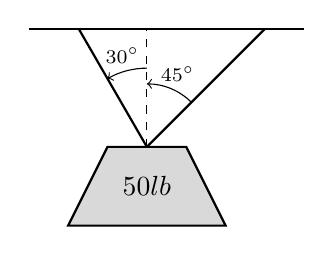
\begin{tikzpicture}
      \filldraw[thick,black,fill=gray!30] (-.5,0) -- (.5,0) -- (1,-1) -- (-1,-1)--cycle;
      \draw (0,-.5) node {$50\unit{lb}$};
      
      \draw [thick] (-1.5,1.5) -- (2,1.5);
      \clip (-1.5,1.5) rectangle (2,-1.25);
      \draw [thick,rotate=120] (0,0) -- (3,0);
      \draw [thick,rotate=45] (0,0) -- (3,0);
      \draw [dashed] (0,0) -- (0,2);
      \draw [rotate=45,->] (.8,0) arc (0:45:.8);
      \draw [rotate=67] (1,0) node {\scriptsize $45^\circ$};
      \draw [rotate=90,->] (1,0) arc (0:30:1);
      \draw [rotate=105] (1.2,0) node {\scriptsize $30^\circ$};
    \end{tikzpicture}
  \end{image}
  One chain makes an angle of $30^\circ$ with the vertical, and the
  other an angle of $45^\circ$. Find the magnitude of the force
  applied to each chain.
  \begin{explanation}
    Start by converting all angles to be measured from the horizontal:
    \begin{image}
      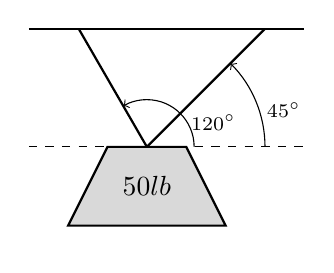
\begin{tikzpicture}
      \filldraw[thick,black,fill=gray!30] (-.5,0) -- (.5,0) -- (1,-1) -- (-1,-1)--cycle;
      \draw (0,-.5) node {$50\unit{lb}$};
      
      \draw [thick] (-1.5,1.5) -- (2,1.5);
      \clip (-1.5,1.5) rectangle (2,-1.25);
      \draw [thick,rotate=120] (0,0) -- (3,0);
      \draw [thick,rotate=45] (0,0) -- (3,0);
      %\draw [dashed] (0,0) -- (0,2);
      %\draw [rotate=45,->] (.8,0) arc (0:45:.8);
      %\draw [rotate=67] (1,0) node {\scriptsize $45^\circ$};
      %\draw [rotate=90,->] (1,0) arc (0:30:1);
      %\draw [rotate=105] (1.2,0) node {\scriptsize $30^\circ$};
      
      \draw [dashed] (-1.5,0) -- (2,0);
      \draw [->] (.6,0) arc (0:120:.6);
      \draw [rotate=20] (.9,0) node {\scriptsize $120^\circ$};
      \draw [->] (1.5,0) arc (0:45:1.5);
      \draw [rotate=15] (1.8,0) node {\scriptsize $45^\circ$};
      \end{tikzpicture}
    \end{image}
    We can view each chain as ``pulling'' the weight up, preventing it
    from falling. We can represent the force from each chain with a
    vector. First, we'll let $\vec{F}_W$ be the force of the weight
    due to gravity.  Since pounds are a unit of force, this is just
    $\vector{\answer[given]{0},\answer[given]{-50}}$.  Let $\vec F_1$
    represent the force from the chain making an angle of $120^\circ$
    with the vertical, and let $\vec F_2$ represent the force from the
    other chain.
    \begin{image}
      \begin{tikzpicture}
      \filldraw[thick,gray!40,fill=gray!20] (-.5,0) -- (.5,0) -- (1,-1) -- (-1,-1)--cycle;

      \draw [very thick,->] (0,0) -- (0,-1.7);
      \draw [very thick,->,rotate=120] (0,0) -- (1.7,0);
      \draw [very thick,->,rotate=45] (0,0) -- (1.7,0);
      
      \draw [->] (.4,0) arc (0:120:.4);
      \draw [->] (1.3,0) arc (0:45:1.3);

      \draw [dashed] (-1.5,0) -- (2,0);
      
      \draw [rotate=20] (.7,0) node {\scriptsize $120^\circ$};
      \draw [rotate=15] (1.8,0) node {\scriptsize $45^\circ$};

      \draw [rotate=120,left] (.85,0) node {\scriptsize $\vec{F}_1$};
      \draw [rotate=50,left] (1,0) node {\scriptsize $\vec{F}_2$};
      \draw [left] (0,-.5) node {\scriptsize $\vec{F}_W = \vector{0,-50}$};
    \end{tikzpicture}
  \end{image}
    Thus
    \[
    \vec F_1 = m_1\vector{\cos(120^\circ),\sin(120^\circ)}
    \]
    \[
    \vec F_2 = m_2\vector{\cos(45^\circ),\sin(45^\circ)}
    \]
    As the weight is not moving, we know the sum of the forces is
    $\vec 0$:
    \[
    \vec F_W + \vec F_1 + \vec F_2 = \vec 0
    \]
    Writing our vectors vertically,
    \begin{align*}
      \begin{bmatrix}
        0\\
        \answer[given]{-50}
      \end{bmatrix}
      +m_1
      \begin{bmatrix}
        \cos\left(\answer[given]{120}^\circ\right)\\
        \sin\left(\answer[given]{120}^\circ\right)
      \end{bmatrix}
      + m_2
      &\begin{bmatrix}
      \cos\left(\answer[given]{45}^\circ\right)\\
      \sin\left(\answer[given]{45}^\circ\right)
      \end{bmatrix}\\
      =
      &\begin{bmatrix}
        \answer[given]{0}\\
        \answer[given]{0}
      \end{bmatrix}
    \end{align*}
    The sum of the entries in the first component is 0, and the sum of
    the entries in the second component is also 0. This leads us to
    the following two equations:
    \begin{align*}
      m_1\cos(120^\circ) + m_2\cos(45^\circ) &=0 \\
      m_1\sin(120^\circ) + m_2\sin(45^\circ) &=50
    \end{align*}
    We leave it to the reader to verify that the solution is:
    \[
    m_1=\answer[given]{50(\sqrt{3}-1)}\unit{lb} \qquad m_2=\answer[given]{\frac{50\sqrt{2}}{1+\sqrt{3}}}\unit{lb}
    \]
  \end{explanation}
\end{example}


%% BADBAD
%% TWO AIRPLANE PROBLEMS
%% One where traveling East relative to ground
%% One where traveling East relative to air


\section{The difference between a point and a vector}

You may be wondering, ``What's the difference between a point and a
vector?'' Here's the deal: A point $P$ specifies \textbf{location}
alone. This location is denoted by an \index{ntuple@$n$-tuple}\index{tuple}$n$-tuple:
\[
P=(p_1,p_2,\dots,p_n)
\]
On the other hand, a vector $\vec{v}$ is also represented by a tuple:
\[
\vec{v} = \vector{v_1,v_2,\dots,v_n}
\]
However, the \textbf{interpretation} of this $n$-tuple is quite different
than that of a point. Here, the tuple represents the location of the
``tip'' of the vector while the ``tail'' of the vector is at the
origin. By thinking of this tuple, $\vec{v}$, as a vector, we can
perform many arithmetic and algebraic properties that we discussed
above. Moreover, it is common to denote points with vectors:
\begin{image}
  \begin{tikzpicture}
	\begin{axis}[
            xmin=-1,xmax=5,ymin=-1,ymax=3,
            clip=false,
            axis lines=center,
            ticks=none,
            unit vector ratio*=1 1 1,
            xlabel=$x$, ylabel=$y$,
            %ytick={-2,-1,...,7},
	    %xtick={-2,-1,...,10},
	    %grid = major,
            every axis y label/.style={at=(current axis.above origin),anchor=south},
            every axis x label/.style={at=(current axis.right of origin),anchor=west},
          ]
          \addplot[mark=*,penColor2] coordinates {(4,2)};
          \node[above] at (axis cs:4, 2) [penColor2] {$(a,b)$};
          \addplot[ultra thick, penColor,->] plot coordinates {(0,0) (4,2)};
          \node[above] at (axis cs:2, 1) [penColor] {$\vector{a,b}$};
        \end{axis}
\end{tikzpicture}
\end{image}
Since a vector can be represented by an $n$-tuple, we denote a point
by a vector by imagining the tail of the vector as being at the
origin. Placing a vector with its tail at the origin is sometimes
called \index{standard position}\textit{standard position}.


We summarize the arithmetic and algebraic properties of vectors
below.

\begin{theorem}[Properties of Vectors]
The following are true for all scalars $s$ and $t$, and for all
vectors $\vec u$, $\vec v$ and $\vec w$ in
$\R^n$.\index{vector!algebraic properties}
\begin{description}
\item[Commutativity:] $\vec u+\vec v = \vec v+\vec u$.
\item[Associativity:] $(\vec u+\vec v)+\vec w = \vec u+(\vec v+\vec w)$.
\item[Additive identity:] $\vec v+\vec 0 = \vec v$.
\item[Compatibility with scalars:] $(st)\vec v= s(t\vec v) = (ts)\vec{v}$.
\item[Distributivity of scalars over vectors:] $s(\vec u+\vec v) = s\vec u+s\vec v$.
\item[Distributivity of vectors over scalars:] $(s+t)\vec v = s\vec v+t\vec v$.
\item[Scaling of magnitude:] $|s\vec v| = |s|\cdot|\vec v|$.
\item[Definiteness:] $|\vec{u}| = 0$ if and only if $\vec u = \vec 0$.
\end{description}
\end{theorem}
Note, you should not memorize these properties (yet!). Rather, you should be
able to work with vectors, and use these properties when appropriate.

\end{document}
